
\section{Bladder cancer} \label{s:lit:biology}

\vspace{3mm}
% \noindent\rule{17cm}{0.2pt}
\fbox {
    \parbox{\linewidth}{
      \begin{itemize}
        \item Introduction to cancer and bladder cancer
        \item Presenting the existing MIBC classifiers
      \end{itemize}
    }
}
\vspace{3mm}

\subsection{What is cancer?}

To understand cancer, we need to know how cells work and replicate in tissues, which is only possible by studying the constituent blocks that are represented or regulated by proteins, which in turn are created by the instructions from \acrfull{dna}. To find the faulty biological processes the analysis needs to be performed on both the malignant and healthy cells/tissue enabling the comparison between normal and abnormal behaviour. To do this, scientists use multiple streams of information from molecular biology which includes gene expression (transcriptomics), mutations (genomics), and proteomics. \textit{In vitro} and \textit{in situ} experiments targeted on a single gene or set of genes, provide additional and invaluable information about the biology of a tissue. By combining biological knowledge with computational modelling, researchers are creating representations such as gene interactions networks or gene pathways. 

% introduction to DNA & RNA, the genetic diversity on Earth, why it's important and some fascinating facts
A useful analogy for engineers is that a \acrshort{dna} molecule is the equivalent of a hard drive where information is stored, while the \acrfull{rna} is similar to \acrfull{ram}. This represents the relevant information (from the DNA) needed to make new copies of a particular protein. Even though all the living organisms share a large amount of DNA, each species has its features\footnote{Interestingly the same mechanism to build proteins is present in animals, plants and is highly similar in bacteria and other living organisms.}. Across a species, the genetic material varies slightly, making the individual both unique and ordinary, depending on the reference point. At conception, the cells of an individual share the same genetic information, but as it ages, the new cells created will start to have anomalies specific to the tissue. Cellular proliferation is tightly regulated, but some of these accumulated anomalies may cause uncontrolled proliferation, leading to tumours. A benign tumour keeps growing without invading the nearby cells while the malignant ones spread across the tissue and invade throughout the body, when it becomes metastasis. 

\begin{figure}[!htb]
  \centering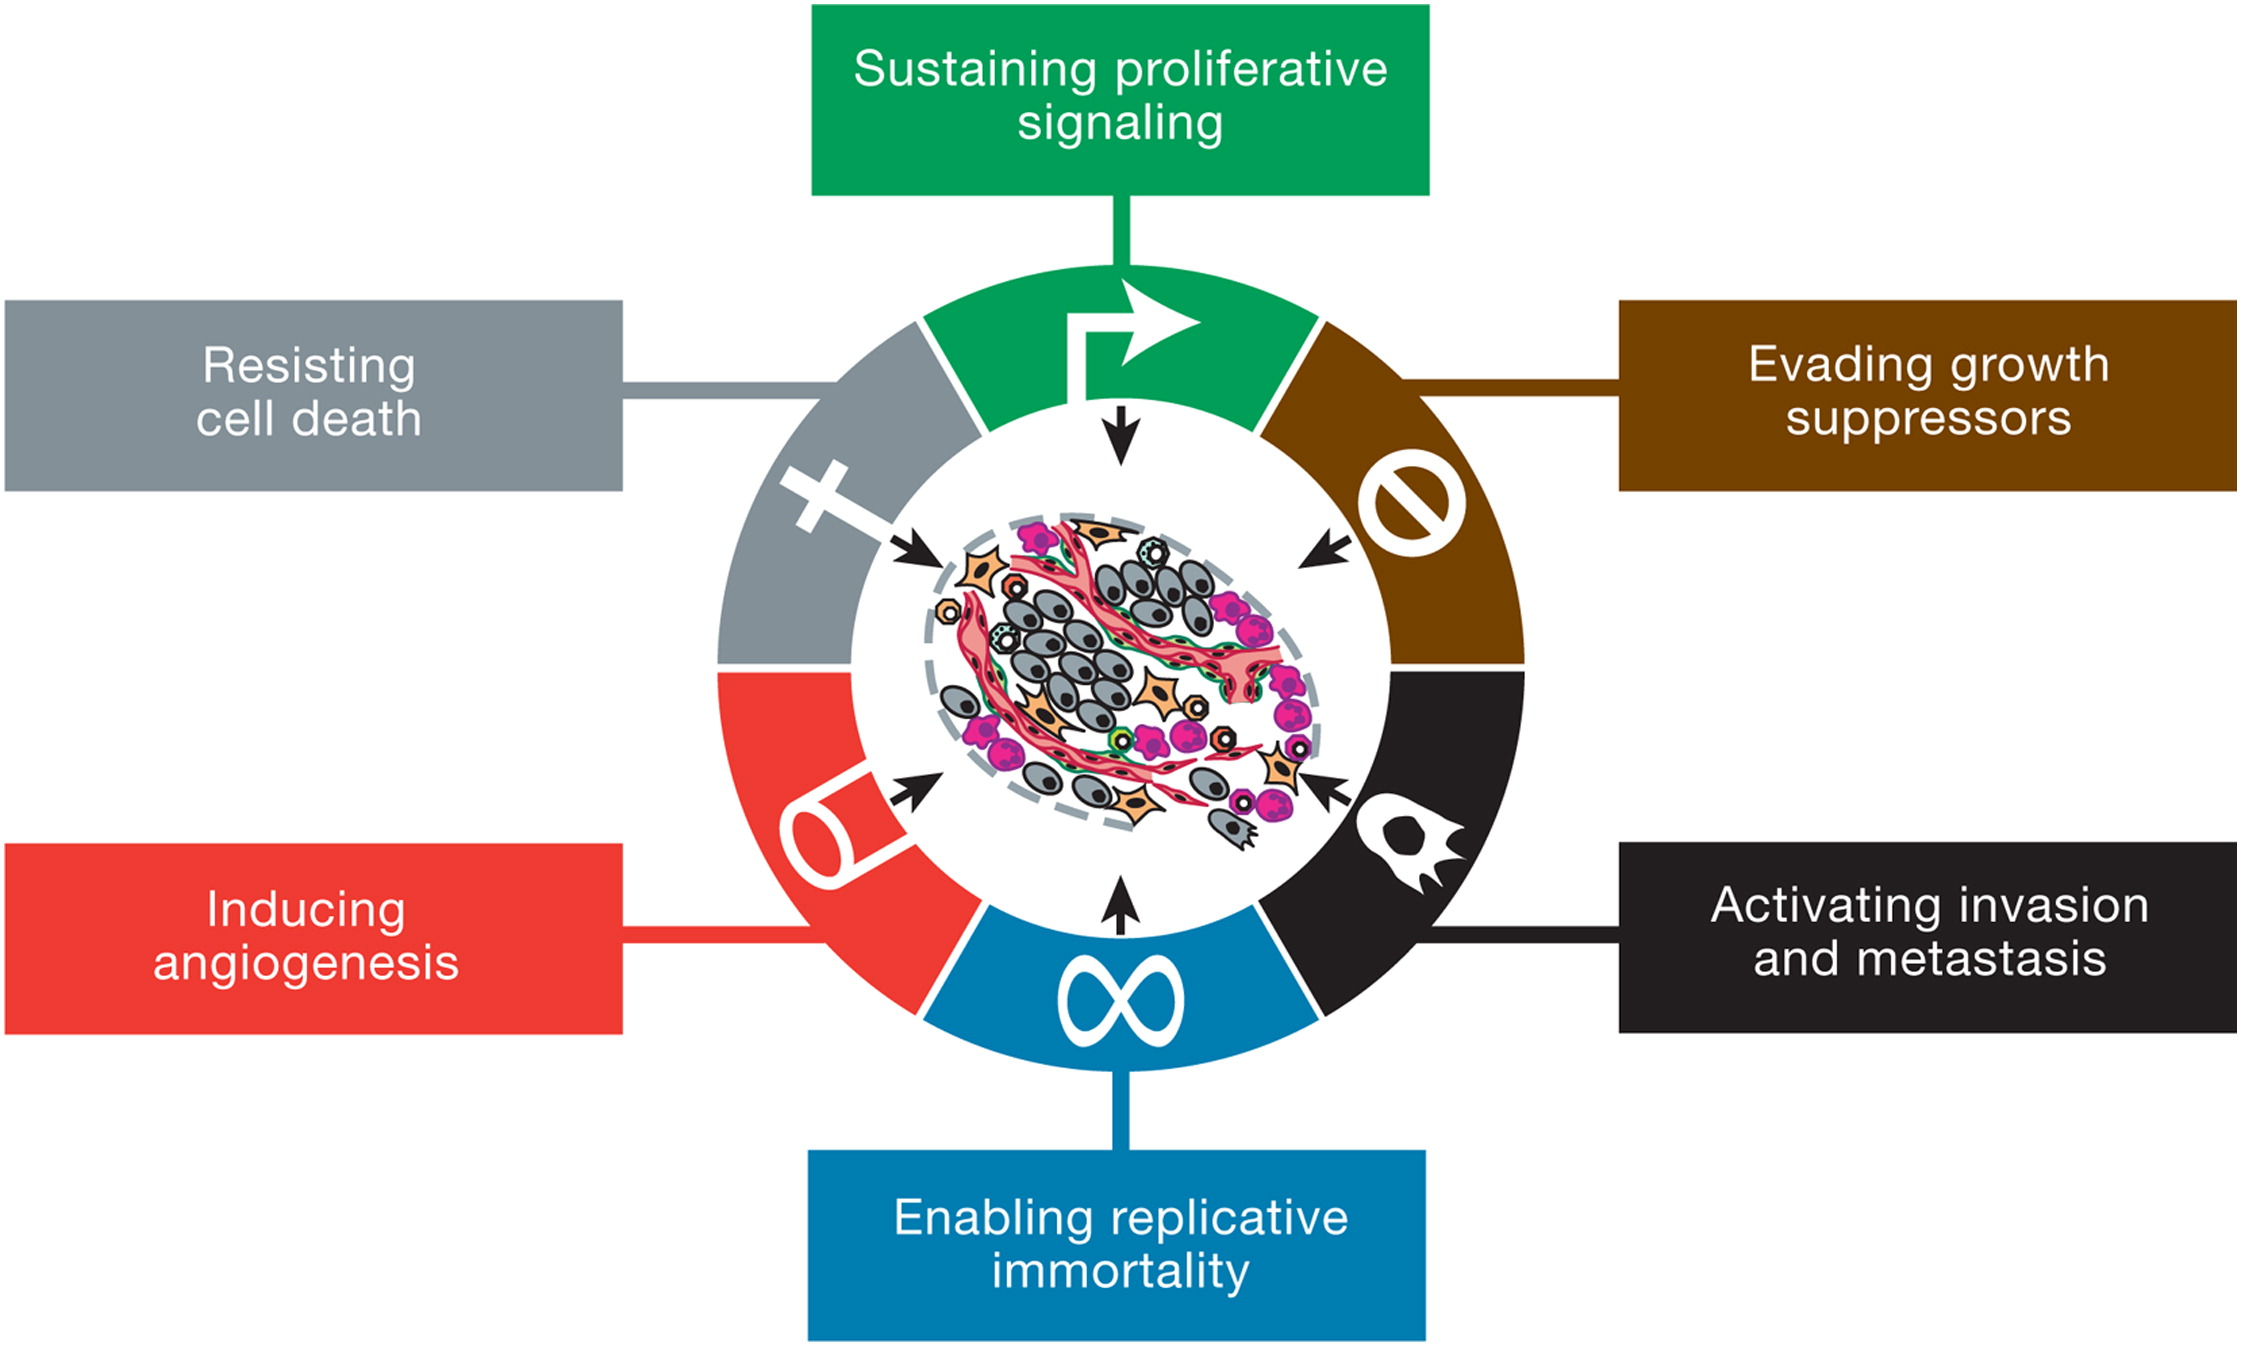
\includegraphics[width=0.8\textwidth,height=0.8\textheight,keepaspectratio]{Sections/Lit_review/Resources/tumour_causes.jpeg}
    \caption[Hallmarks of the tumours]{Hallmarks for tumours from \citep{Hanahan2011-px}. The Sustaining proliferative signalling feature means that the cancerous cell will be "encouraged" to divide while evading the growth suppressors and resist cell death will only aid the birth of new malign cells. Additionally, these cells have the replicative immortality trait. Activating invasion and metastasis means that the cells are capable of spreading to other parts of the body. Finally, angiogenesis refers to the tumours capability to draw nutrients to sustain itself through the creation of blood vessels. }
    \label{fig:hallmarks_cancer}
\end{figure}

% Small paragraph showing the ideas
% Numerous sources are causing genetic alterations in a healthy organism which can lead to diseases. \Cref{fig:hallmarks_cancer} from \citep{Hanahan2011-px} shows that a large proportion of the tumour hallmarks are related to the cell division cycle due to the properties of a cell. This is the one that comes under most natural selection because it leads to growth and/or expansion of the tumour. From evading growth suppressors to resisting cell death, the cancerous cell will not stop dividing, bypassing the tissue population size control, and will slowly conquer the tissue as the healthy cells will reach the end of their cycle and die.

% Comment on the cancer hallmarks
Numerous sources cause genetic alteration in a healthy organism which can lead to disease. In a review of the cancer hallmarks \citep{Hanahan2011-px} there are six different aspects that contribute to tumour malignancy, summarised in \cref{fig:hallmarks_cancer}.  Dis-regulation in the homeostasis of the tissue ("Resisting cell death",  "Sustaining proliferative signalling", 'Evading growth suppressors", "Enabling replicative immortality") combined with cell invasion and angiogenesis (formation of blood vessels) lead to malignant tumours. 

A driving motivation in cancer research is to understand the gene mechanisms in order to develop a cure for the disease. Medicine has made significant progress in cancer research and diagnosis, but the disease generally remains an unsolved problem. One of the reasons for this is the complexity of gene interactions. Another reason, which follows from the first, is the challenge of feasibility. It is not feasible to collect the ideal data\footnote{The ideal genomic dataset would consist of a large number of tumour samples, matched with blood samples, and sequenced across multiple omics (proteins, RNA, mutations, etc.). Multiple samples from the same donor would be needed to track genetic changes as the disease progresses and to map these changes to the appropriate genes.} necessary to create an accurate molecular representation of the disease's evolution. Due to ethical and clinical considerations, samples are typically taken at the time of cancer surgery, making repeated biopsies impractical. Additionally, forming a molecular representation of normal tissue is nearly impossible due to the invasive nature of collecting the necessary data. Consequently, it is challenging to determine the exact gene interactions that drive a specific cancer. A central part of this project is to build such a representation enabling the analysis of genes interactions and linking these to the previously derived subtypes. Some of the existing methods are covered in \cref{s:lit:nets_bio} and the network pipeline developed in the project in \cref{s:N_I,s:N_II}.

This project addresses the challenges of building a more accurate molecular representation of bladder cancer by integrating both tumour and healthy dataset, as presented in \cref{s:N_II}. Using networks/graphs also helps represent gene interactions based on RNAseq expression data. Integrating mutations into the network highlights potential anomalies in molecular processes, while the inclusion of \acrshort{tf} enhances the regulatory understanding of a subset of genes. Although forming an integrated representation of the available molecular information provides a closer approximation to biology, it increases the system's complexity. As highlighted in the following sections, this approach differs from previous research in stratifying bladder cancer.


Before delving into the integration of multi-omics data, bladder cancer needs to be introduced with its molecular characteristics and its impact on the world's population.


% Bladder cancer
\subsection{Bladder Cancer} \label{s:lit:bladder_cancer}

% Overview of the bladder cancer stats
According to Cancer Research UK, bladder cancer is the 9th most common cause of cancer death and the 11th most common cancer in the UK (\citeyear{Cancer_Research_UK2015-cf}). This is equivalent to $\sim$10,000 diagnosed cases per year from which  $\sim$5000 are deaths, with a 5-year survival rate of 52.6\%. In 2008 the global estimate for bladder cancer was $\sim$380,000 new cases and $\sim$150,000 deaths per year \citep{Ferlay2010-sx}. In 2020, there were $\sim$573,000 cases with $\sim$212,536 deaths reported, which shows a considerable increase in cancer cases\footnote{A good resource to get an overview of the prevalence of bladder cancer (and other cancers too) is the \href{https://gco.iarc.fr/en}{website} from World Health Organisation, particularly the trends in cancer overtime} \citep{Sung2021-hn}. 

% Focuse on urotheliam carcinoma
In the population across Northern and sub-Saharan Africa, there is a particular pattern in bladder cancer incidence caused by infection with the parasitic worm \textit{Schistosoma} and other occupational risks \citep{Ferlay2010-sx}. Unfortunately, there is not enough available molecular data to study these cases, and this project is concerned with \acrfull{uc}, which typically affects men from Western countries who are three times more likely to develop bladder cancer \citep{Knowles2015-mu}.
 

% Talk about bladder cancer causes, economical burden
Ageing is one of the main risk of bladder cancer representing more than half of the new cases (\citeyear{Cancer_Research_UK2015-cf}), smoking is another factor that is attributed to the disease \citep{Knowles2015-mu} however there is no mechanism link between smoking and bladder as it is with lung cancer. Other environment risk factors include metal contamination, usually found in arsenic-water, or exposure to ionising radiation reviewed by \citep{Knowles2015-mu}. 

% Types ands stages of bladder cancer
Several systems have been used to classify bladder depending on their utility. For medical doctors, there are two popular systems to dichotomise the bladder cancer: Tumour-Node-Metastasis (TNM) and the International Society of Urological Pathology (ISUP), Figure 1 from the bladder cancer review \citep{Knowles2015-mu} is a good visual representation of the stages\footnote{Link to \href{https://www.nature.com/articles/nrc3817/figures/1}{Figure 1} from the bladder cancer review \citep{Knowles2015-mu}.}. The figure is an illustration of the stages and their classification, though is not representative of the bladder cancer progression.


There are two main types of bladder cancer: \acrfull{nmibc} and \acrfull{mibc}. Stages Tis, Ta, and T1 are classified as NMIBC, as they have not invaded the muscle\footnote{Check \href{https://www.nature.com/articles/nrc3817/figures/1}{Figure 1} from the bladder cancer review \citep{Knowles2015-mu} for a good visual representation of the stages.}. At first presentation, approximately 70\% of bladder cancer patients are found to have \acrshort{nmibc}, with a 5-year survival rate of around 90\%. Although surgical resection is often successful, the disease frequently recurs in 50-70\% of cases, with only 10-15\% progressing to muscle invasion \citep{Knowles2015-mu}. At the time of writing, it is not possible to determine which recurrent cases will progress to \acrshort{mibc}. Patients with \acrshort{nmibc} generally have favourable prognoses, although their quality of life is impacted by the need for regular cystoscopic checkups to preempt the progression of the disease into muscle-invasive bladder cancer. The routine medical checkups contribute to the expensiveness of bladder cancer treatment, adding an economic burden on both the healthcare system and the patients.

The muscle invasive bladder cancer encompasses the T2a, T2b, T3 and T4 stages and it appears in $\sim$30\% of the bladder cancer cases. It is more aggressive than the NMIBC, with $\sim$50\% chances of 5-year survival. Almost half of the cases of MIBC develop metastasis and for these patients the median survival is 12-15 months \citep{Knowles2015-mu}. Usually the metastatic sites for bladder cancer are lungs, livers and bones.

Even though the \acrshort{mibc} and \acrshort{nmibc} are bladder cancer, their form and treatment differs. Patients with the more aggressive MIBC undergo cystectomy, a procedure whereby the entire bladder is removed, while NIMBC patients have \acrfull{turbt} followed by regular cystoscopies checkups. Both procedures negatively impact the patients' quality of life. Developing better diagnosis, tools and treatment plans for bladder cancer, especially for the MIBC, is therefore imperative. As the following sections (\cref{s:lit:subtypes_mibc}) will show the MIBC is a heterogeneous and complex disease with high mutation burden, covered in \cref{s:lit:bladder_other}. It is the aim of this project to build on the research that has been done so far in bladder cancer in order to develop better ways of subtyping it, focusing particularly on the MIBC.

\subsection{MIBC subtyping} \label{s:lit:subtypes_mibc}

% I would insert a bit of history here, before the "culminated" bit.
% Talk about how initially they were grouped into 2 main groups based on diff/aggressiveness. Then how increasing cohort size facilitated finer definition, but led to slightly contrasting classifications, unified in a consensus.
% Could also make a statement around consensus suggesting "finished" but how that is so not true.

To better understand \gls{MIBC} and develop targeted treatments, significant research was undertaken to subgroup the disease. In one of the first attempts to stratify MIBC by gene expression, \citet{Choi2014-ed} identified three subgroups, basal, luminal, and \textit{p53}, in a cohort of 73 samples. In the same year, the first gene expression analysis of the initial 131 samples from the \gls{TCGA} MIBC cohort was published, identifying four subgroups, with the basal and luminal trends similar to \citet{Choi2014-ed}. As more RNAseq data became available, MIBC became increasingly studied, culminating in the consensus work \citep{Kamoun2020-tj}.


This section covers three main studies on \acrshort{mibc} stratification, the work from \acrshort{tcga} \citep{Robertson2017-mg}, Lund group \citep{Marzouka2018-ge} and the MIBC consensus \citep{Kamoun2020-tj}. These three studies are particularly important for this project as TCGA is the main tumour dataset used and the consensus is the referential classification on MIBC research. The subtypes derived by the Lund group have been used to verify the results in this project against a non-TCGA based group.

There are two main components of each study that are relevant for this project: the methods used for clustering the gene expression and the biological output. Despite the consensus work combining multiple studies, TCGA and the Lund classifications maintain their relevance by offering a list of genes specific to each subtype. 

\begin{figure}[!htb]   
\centering
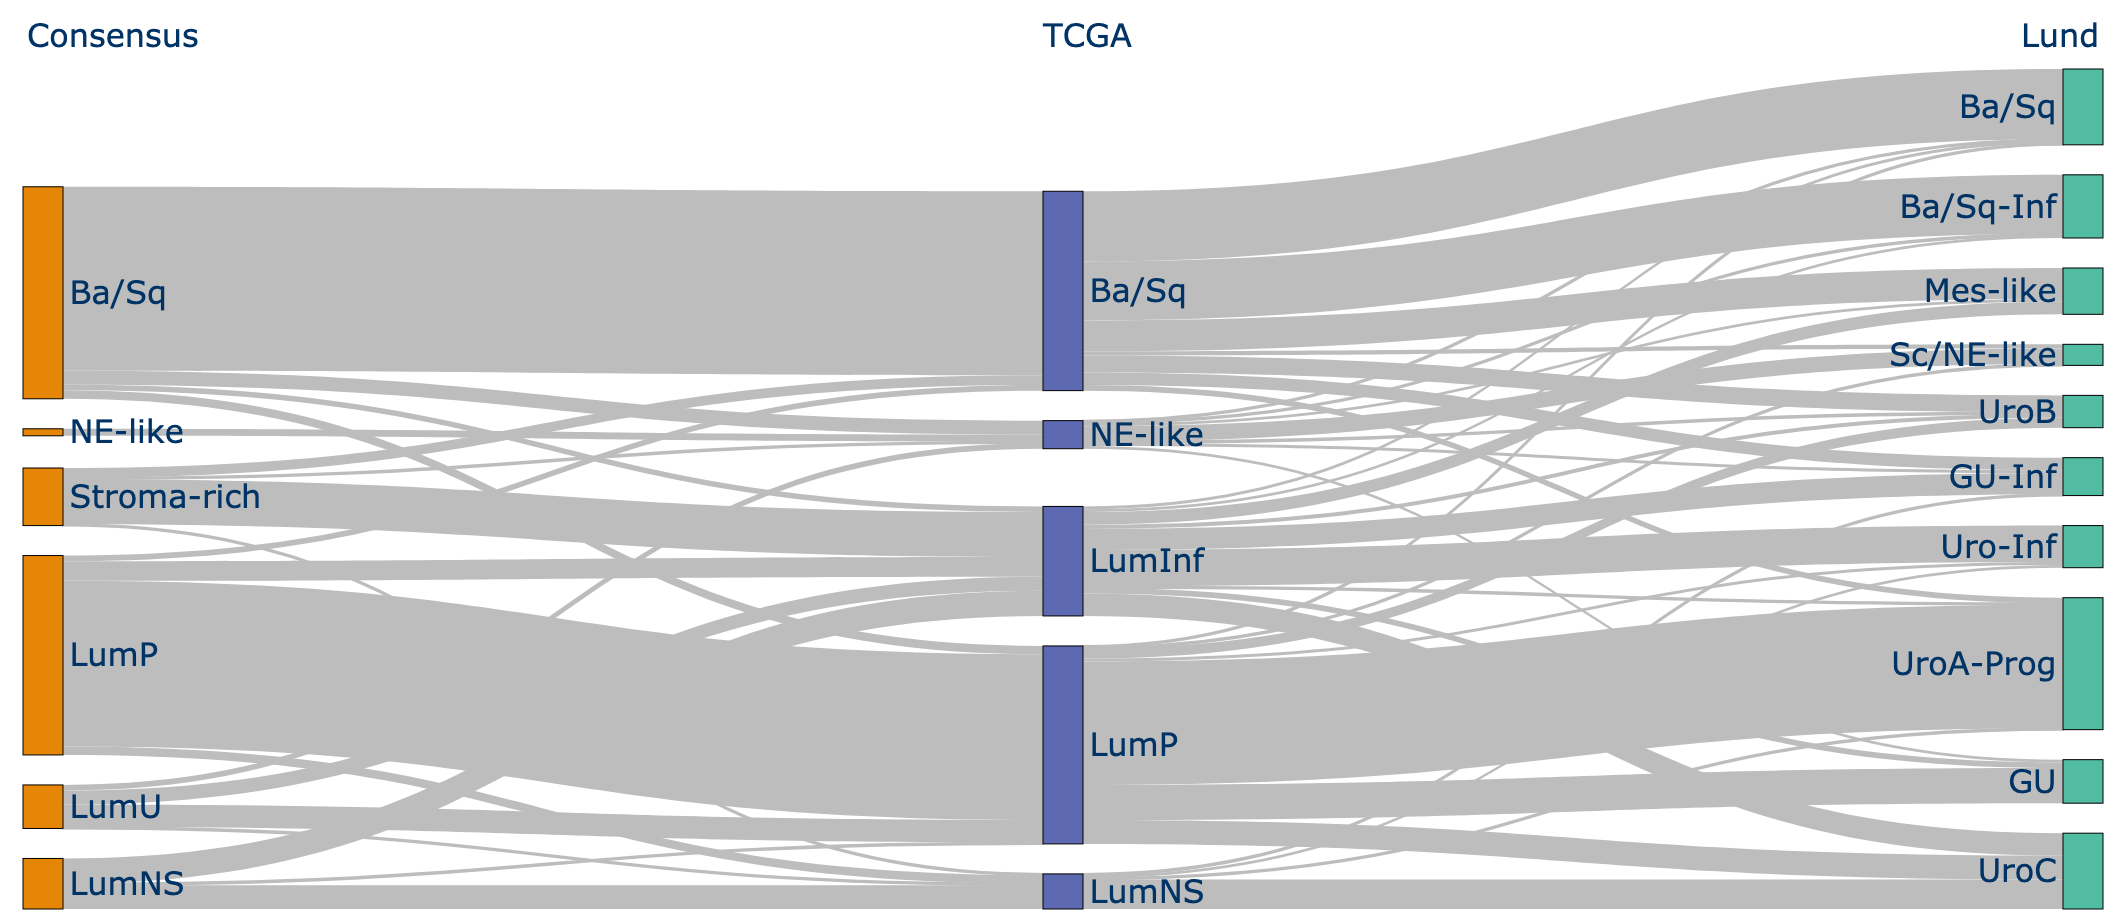
\includegraphics[width=1.0\textwidth,height=1.0\textheight,keepaspectratio]{Sections/Lit_review/Resources/classifier_differences.png}
  \caption[Comparison between existing MIBC classifications]{Sankey plot showing the differences between the consensus \citep{Kamoun2020-tj}, TCGA \citep{Robertson2017-mg} and Lund \citep{Marzouka2018-ge} classifications of the MIBC.}
\label{fig:lit:classifier_comp}
\end{figure}

The Sankey plot (\cref{fig:lit:classifier_comp}) shows the difference in sample classifications across the three studies covered in this project. The consensus and TCGA subgroups are fairly consistent with each other, the major difference being the \acrfull{luminf} group being split into \acrfull{stroma}, \acrfull{lumu} and \acrfull{lumns} by the consensus. However, the Lund group has more subtypes, splitting the Basal into three smaller subtypes, the \acrfull{ba/sq}, Ba/Sq infiltrated and \acrfull{ba/sq}. The Luminal group is also named Urothelial-like and contains the \acrfull{gu} gorups. Both Lund and TCGA groups are part of the consensus work, but given the large difference between the Lund and the other two classifications, it can be notice which classification had a larger influence in the consensus.


% TCGA
\subsubsection*{TCGA} \label{s:lit:tcga_mibc}

% Introduction of TCGA
The MIBC cohort from TCGA is an invaluable asset for the research community as a number of sequencing techniques have been applied to the samples: mRNAseq (gene expression), \acrfull{wes}, microarray-based (copy number variations) as well as metadata about the patients. This cohort is characterised by aggressive tumours, having a high grade of muscle invasion and contains 412 tumour samples. There are two comprehensive studies of the \acrlong{tcga} cohort from \citet{Tcga2014-dr} and \citet{Robertson2017-mg}. The former constitutes the research analysing the first batch of patient samples (131) while the latter examines the entire cohort of 412 patient samples. 

In \citep{Robertson2017-mg}, at the pre-processing stage of the RNAseq data, the under-expressed genes were removed, and only the 25\% with the highest standard deviation were selected, reducing the number of genes to 3347. This is followed by a dimension reduction step where the authors used the Bayesian approach \acrfull{nmf} \citep{Schmidt2009-zh}. \citet{Robertson2017-mg} then use agglomerative hierarchical clustering with average linkage and found five clusters.

% Talk about TCGA subtypes
In the work of \citet{Robertson2017-mg} multiple data types are analysed separately, centring on the subgroups derived from gene expression and then correlating them with the other data analysis. The main result is the stratification of the MIBC into five distinct molecular subtypes: $35\%$- \acrfull{lump}, $19\%$ \acrfull{luminf}, $6\%$ \acrfull{lum}, $35\%$ \acrfull{ba/sq} and $5\%$ \acrfull{ne}. The highest 5-year survival is given by the Luminal subgroups while the Neuronal has the least favourable prognosis. 

The work of \citet{Robertson2017-mg} offers a comprehensive description of the genes that are expressed in their MIBC stratification. The molecular subtypes, the genes specific of the subgroups and their function, are presented in \cref{tab:lit:tcga_genes}. Figure 2 from their paper shows the RNASeq heatmap for the MIBC subtype genes and also features in the appendix \cref{fig:ap:tcga_subtypes}\footnote{The gene summary and the corresponding figure were presented in the Appendix with the goal to centralised the known gene singatures in the literature. The same was done for Lund and consensus classifier \citep{Marzouka2018-ge,Kamoun2020-tj}.}.


TCGA is the largest cohort from the MIBC consensus and its subtypes are being used in the GUSTO trial presented later on in \cref{s:lit:clinical}. These probably makes TCGA the most influential cohort in the MIBC research. However, due to the heterogeneous nature of the disease and the differences with the Lund classification (uses additional data for subtyping), it is imperative to acknowledge the bias introduced in the MIBC stratification, especially considering that the cohort contains very aggressive tumours.

% Lund
\subsubsection*{Lund} \label{s:lit:lund_mibc}

% Introduce Lund cohort
At Lund University, Sweden, significant efforts have been made by \citep{Sjodahl2017-xr, Marzouka2018-ge} to stratify MIBC. Known as the Lund classifier, the work encompasses 307 aggressive tumour samples on which microarray sequencing was performed to determine gene expression. Apart from the different sequencing technology, what sets the Lund cohort apart is the \acrfull{ihc} matched dataset (mostly) used to inform their previous stratification \citet{Sjodahl2017-xr}, which was based solely on gene expression.

% Clustering approach
As with most studies on cancer stratification based on gene expression, \citet{Sjodahl2017-xr} applied a stepwise hierarchical clustering to the 307 samples, identifying 6 subtypes. This was followed by the work of \citet{Marzouka2018-ge} from the same lab, which used the IHC information to further split the samples into 10 groups and create a classifier\footnote{Precursor of the consensus classifier}. In their later work, the group selected 1200 of the most representative genes of the classes by applying a bootstrapping-like method.

\citeauthor{Marzouka2018-ge} applied their 10 groups classifier on the MIBC cohort from TCGA (\cref{fig:lit:classifier_comp}) founding four Urothelial-like subtypes: UroA-Prog, Uro-Inf, UroB, and UroC; two genomically unstable GU and GU-inf; two \acrfull{ba/sq}  Ba/Sq and Ba/Sq-inf; and two other groups, \acrfull{mes} and \acrfull{sc/ne}. \Cref{fig:lit:lund_fig} from \citet{Marzouka2018-ge} offers a good overview of the specific gene expression for each of the Lund subtypes, and \cref{tab:lit:lund_genes} summarises the highlighted genes for the main groups.

Compared to other classifiers, the Lund group referred to the luminal samples as "Urothelial-like." With the addition of IHC data and tumour purity scores (immune and stromal infiltration), the authors further distinguished subgroups with high cell infiltration by appending the "-inf" suffix; see \cref{fig:lit:classifier_comp} for comparison. The additional information from IHC makes the study an indispensable resource, enriching the understanding of MIBC. Moreover, several scores developed by combining multiple gene expressions assist in stratification. For example, the Basal/Squamous ratio, \textit{ERBB} score, and circuit score are all used to distinguish between luminal and basal, GU and Uro-b, or stromal and basal subtypes (\cref{fig:lit:lund_fig}).

Nevertheless, as with TCGA subtyping, the Lund subgroups are derived mainly from gene expression data and do not incorporate other omics information such as mutations. The uses of the IHC data only enriches the MIBC subtyping, enforcing the hypothesis of the project of integrating multi-omics at the computational level.

\begin{figure}[!t]   
\centering
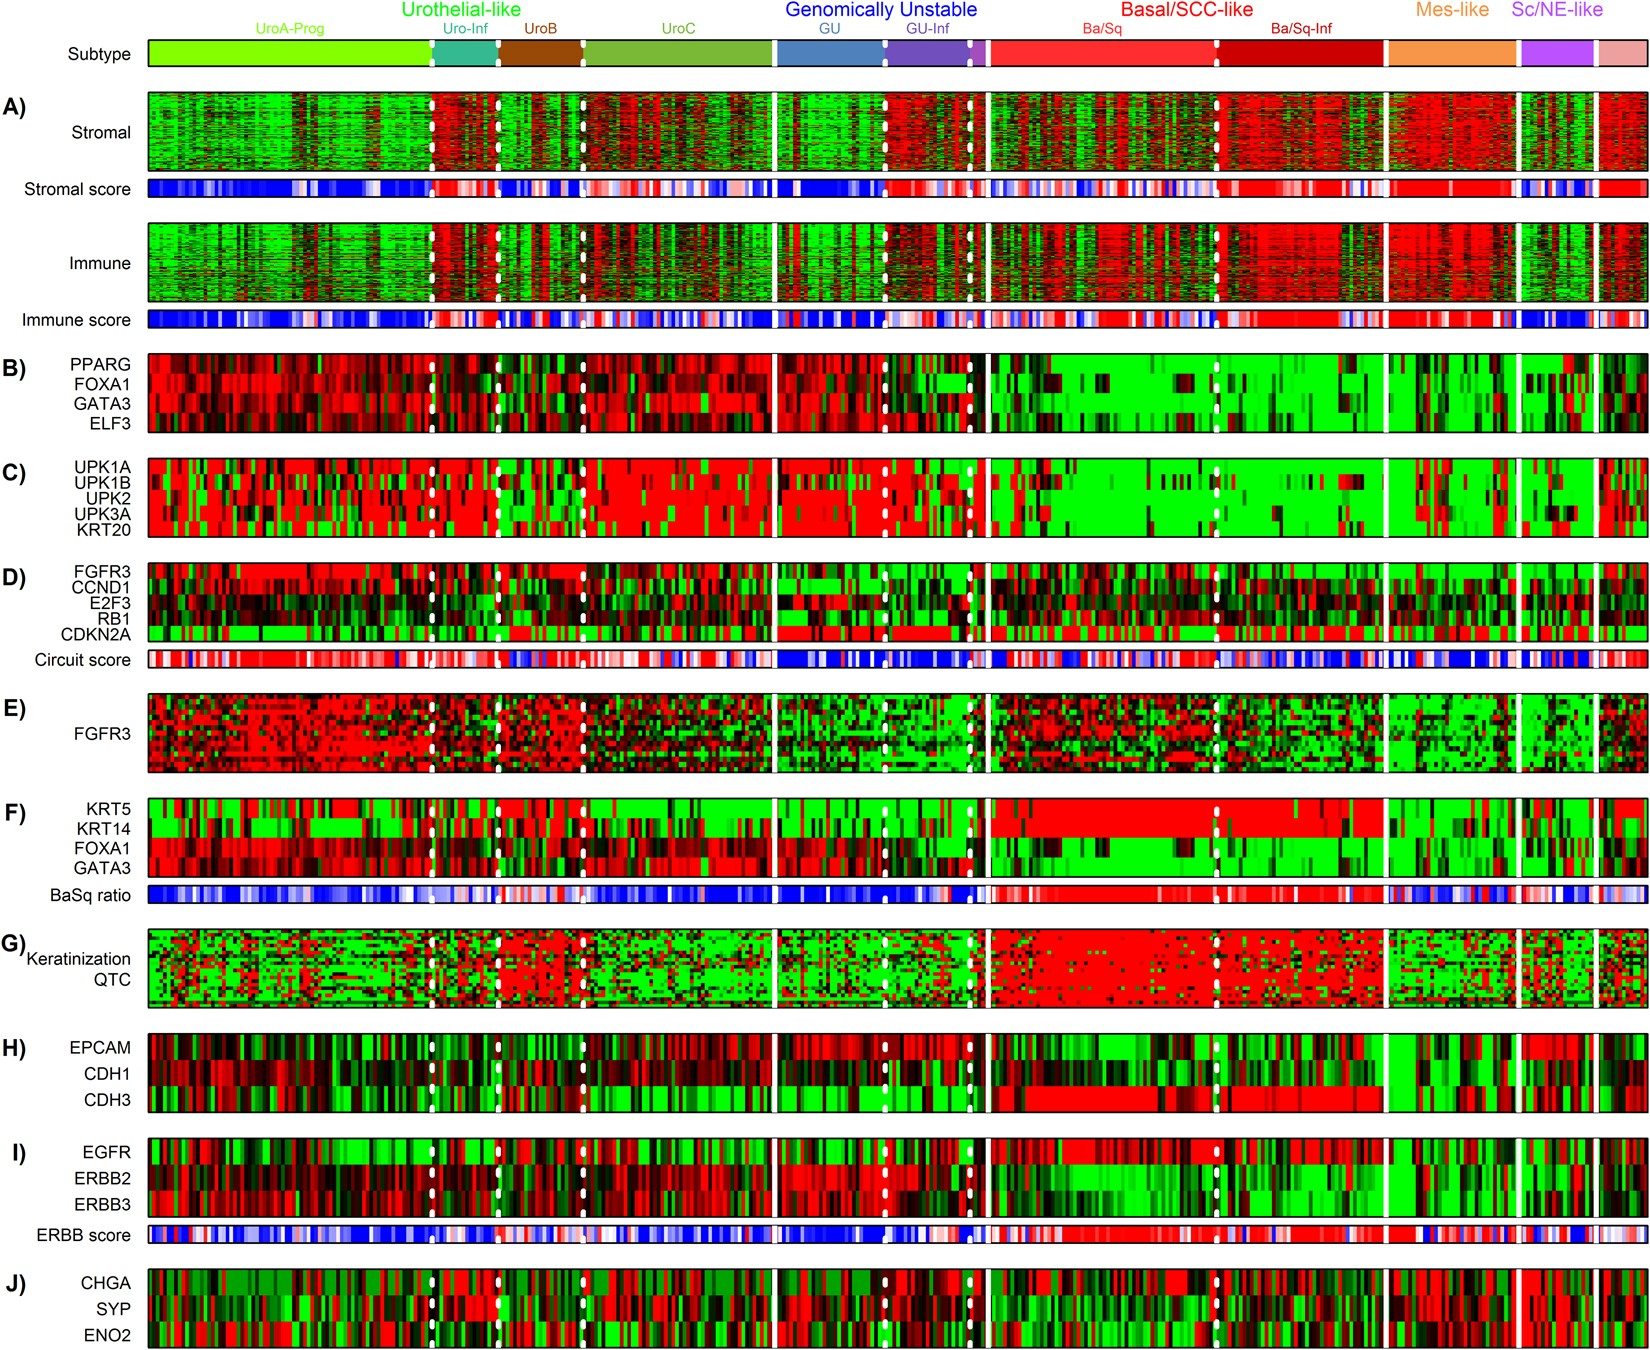
\includegraphics[width=1\textwidth,keepaspectratio]{Sections/Lit_review/Resources/Lung_subtypes.jpg}
  \caption[Summary of MIBC subtypes using Lund classifier]{Subtyping the MIBC cohort from TCGA using the Lund classifier \citep{Marzouka2018-ge}. A) represents the stromal and immune cell signatures as well as the scores computed with the ESTIMATE tool\citep{Yoshihara2013-wq}. B-J represents subtype-specific signature scored as well as the Circuit, \acrshort{ba/sq} ratio and \textit{ERBB} which aids the separation of subtypes. The signature scores are summarised in \cref{tab:lit:lund_genes} and image is reproduced from \citep{Marzouka2018-ge}.
}
\label{fig:lit:lund_fig}
\end{figure}
\FloatBarrier


% Consensus
\subsubsection*{Consensus} \label{s:lit:consensus_mibc}

% Introducing the consensus work
The TCGA and Lund cohorts are part of the research effort from \citet{Kamoun2020-tj} to find a consensus among the multiple studies on MIBC stratifications. There are a total of six different cohorts used in the consensus, and except for the two already mentioned \citep{Kamoun2020-tj}, it also utilises the work of \citep{Mo2018-rl, Damrauer2014-tc, Choi2014-ed, Rebouissou2014-ep}. This resulted in 6 subtypes with their molecular characteristics, see \cref{fig:lit:2020_consens}. It can be noticed that some subtypes are more prevalent than others, with \acrfull{lump} (24\%) and \acrlong{ba/sq} (35\%) being the most common, followed by \acrlong{lum} and \acrlong{stroma} (both 15\%). Moreover, each subtype has a different mutation signature, which enforces the project hypothesis by adding mutation to the RNAseq data, thus yielding better cancer classifications.

% Present the goal of the paper, the challenge of combining multiple datasets 
There are several points worth emphasising in the consensus paper. The first is that all the approaches used \gls{HIERARCHICAL CLUSTERING} to analyse the gene expression \citep{Mo2018-rl, Damrauer2014-tc, Choi2014-ed, Marzouka2018-ge, Rebouissou2014-ep,Robertson2017-mg}. The second is that all models receive only RNAseq data\footnote{In the work of \citeauthor{Robertson2017-mg} use domain knowledge to choose the number of subtypes.} and the studies are not using the same method to obtain the gene expression (except \citet{Robertson2017-mg, Mo2018-rl} which both are using TCGA data). One consequence of using different data sources is that each study proposed a different set of subgroups. 

% Solution and inspiration from colorectal research
To reach the consensus on subtyping, \citeauthor{Kamoun2020-tj} combined all the datasets resulting in 1750 samples and run the models enlisted above. The output from the approaches listed above was analysed together as a network, using the methods presented in the colorectal consensus work \citep{Guinney2015-fy}. Markov Clustering (MCL - \citet{Van_Dongen2008-yj}) community detection algorithm\footnote{Community detection algorithms play a central role in the methods developed in this PhD and are covered later on in the thesis (\cref{s:lit:comm_detect}).} is applied  across the MIBC cohorts to find the shared subtypes which resulted in six different subtypes as seen in \cref{fig:lit:consensus_network}. 

% To find how the groups of the MIBC subtypes across the classifications Markov Clustering algorithm (MCL) \citet{Van_Dongen2008-yj} is used; this is a type of community detection algorithm, an idea I will return to later in the thesis in \cref{s:lit:comm_detect}. The resultant network can be seen in \cref{fig:lit:consensus_network}.

% Limitations: Small size compared to colorectal; they haven't used other consensus algorithms
One of the consensus limitations (acknowledged by the authors) is the variability of the cohorts and their subtype. The MIBC has 1750 samples compared to 4151 samples used in the colorectal cancer consensus work \citep{Guinney2015-fy}, which represents the initial effort to combine multiple disease classifiers. Running the clustering independently on each separate cohort and not as one combined single cohort was another trade-off imposed by the different sequencing technologies present in the data. 

The main output of the MIBC consensus is an R package\footnote{See the \url{https://github.com/cit-bioinfo/consensusMIBC}.} that can classify a tissue sample based on the expression of 857 genes which were found to cover the properties of the six consensus MIBC subtypes. The subset genes was selected by the statistical test LIMMA moderate t-tests\footnote{For more details check section 'Single-sample transcriptomic classifier construction' from the Supplementary document of the consensus. Alternatives approaches for classifications have been discussed by \citet{Eriksson2022-vw}}. The centroids represent the mean value of these genes across the six different datasets used. For each sample to classify, the Pearson correlation is computed and the column (i.e. consensus subtype) with the highest value represents the MIBC group; if the Pearson correlation is $<$0.2 the samples remains unclassified. 

\begin{figure}[!t]   
\centering
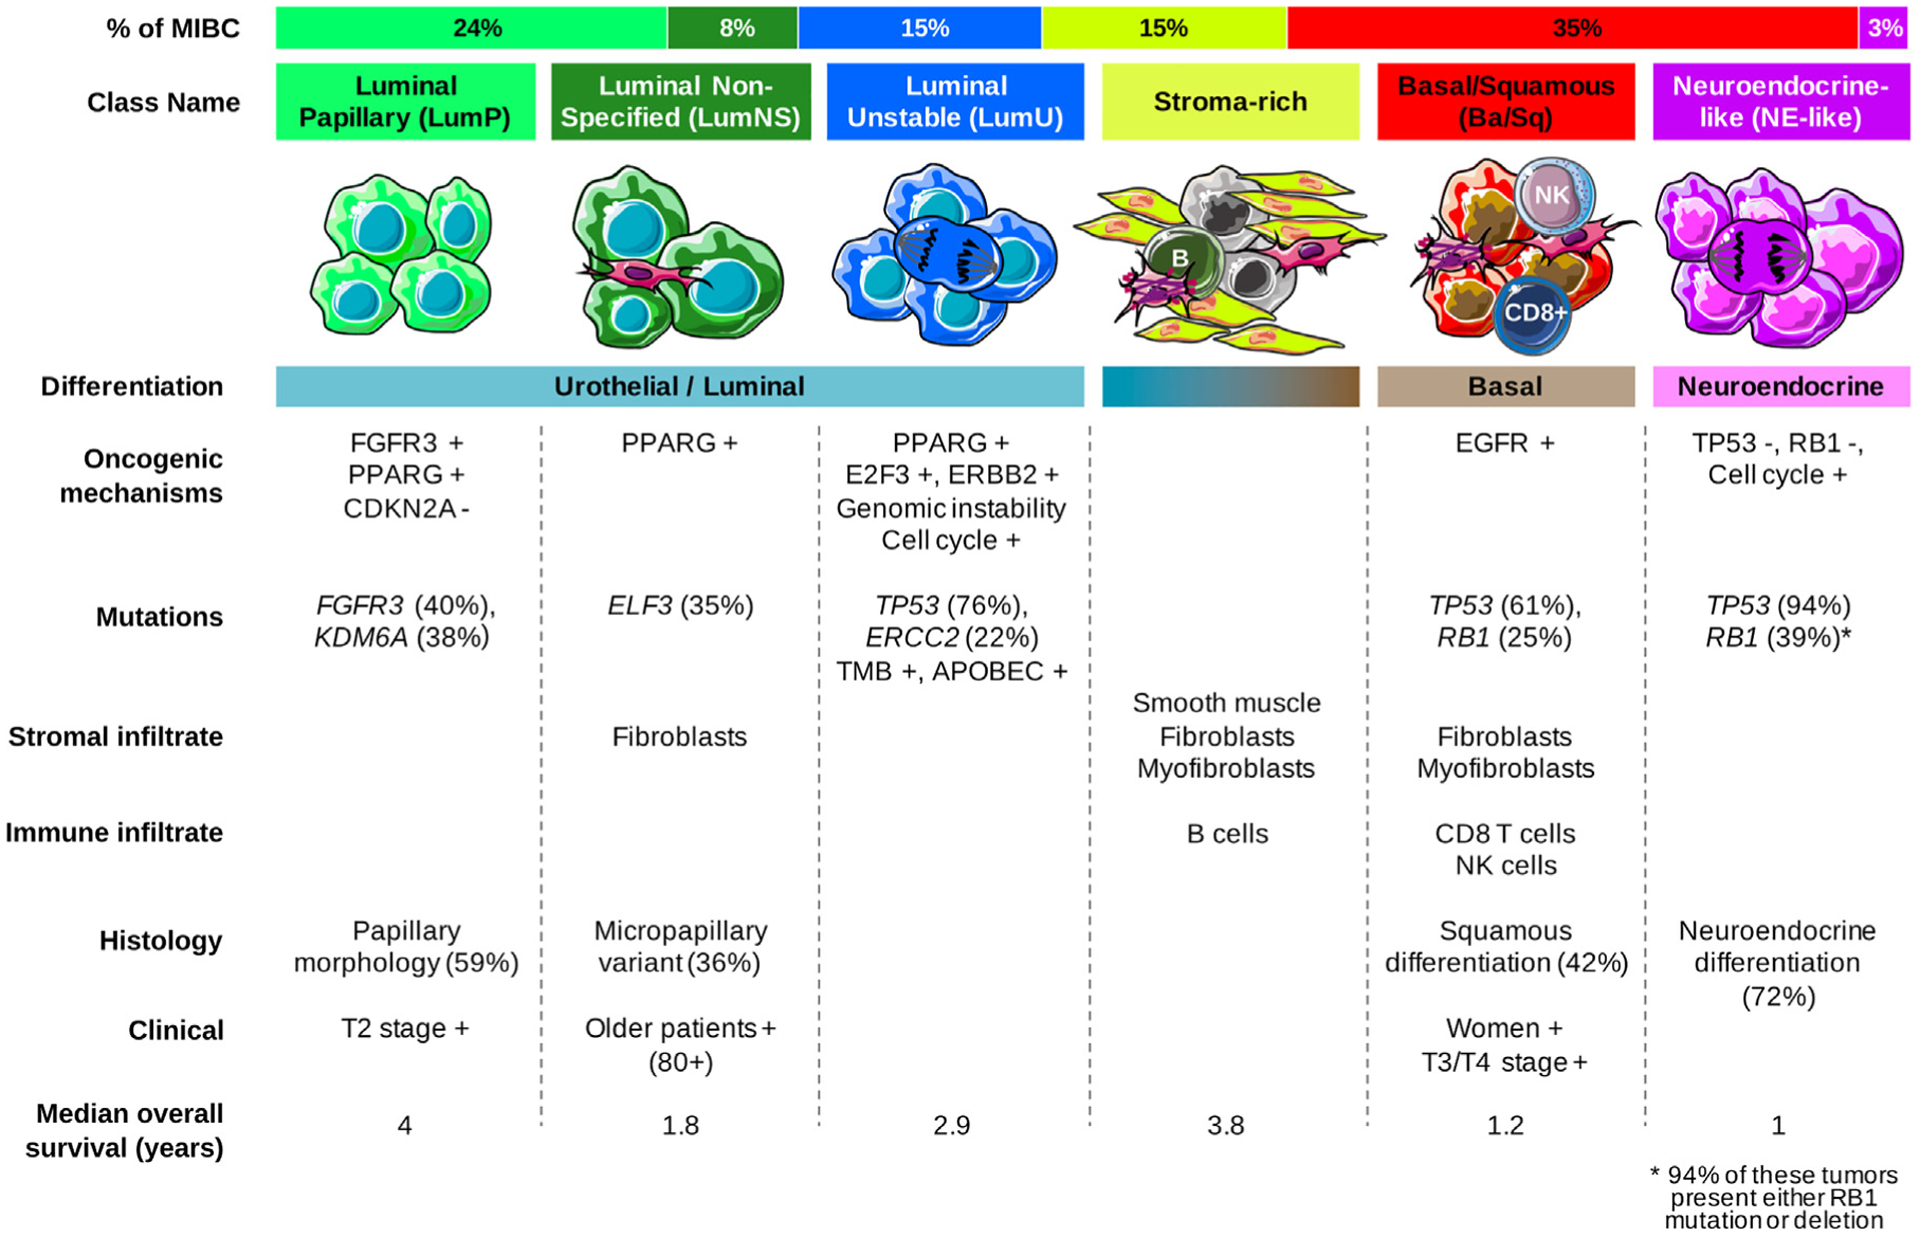
\includegraphics[width=1.0\textwidth,height=1.0\textheight,keepaspectratio]{Sections/Lit_review/Resources/2020_consensus_subtypes.jpg}
  \caption[Summary of the MIBC consensus subgroups]{The six different subtypes of \acrfull{mibc} by the consensus classifier \citep{Kamoun2020-tj}, the names are based on their differentiation status, morphology etc. There are three different types of Luminal Bladder cancer: most common being the ones related to papillary morphology (\acrfull{lump}), \acrfull{lumns} showing immune markers, and \acrfull{lumu} is the new luminal subtype. \acrfull{ba/sq} is the most common bladder cancer and is related to the Squamous tissue. \acrfull{ne-like} share similarities with Ba/Sq cancer and Stroma-rich are likely not to be a biological group but a collection of samples that contain artefacts from the collection or/and other intermediate processes. Image reproduced from \citep{Kamoun2020-tj}.
}
\label{fig:lit:2020_consens}
\end{figure}
\FloatBarrier


TCGA and Lund studies offered a list of the genes specific to each subtype which were summarised in two \cref{tab:lit:tcga_genes,tab:lit:lund_genes} from appendix. In contrast, the MIBC consensus does not provide a clearly defined list of genes specific to each subtype, but a classification tool based on selected genes and a summary of the molecular properties as seen in \cref{tab:lit:consensus_genes}. The classification tool is valuable and useful for the bladder cancer research community, though not without its challenges. Given that the lack of a succinct list of genes could be an indirect consequence of the heterogeneity of the disease.


\begin{figure}[!htb]    
    \centering
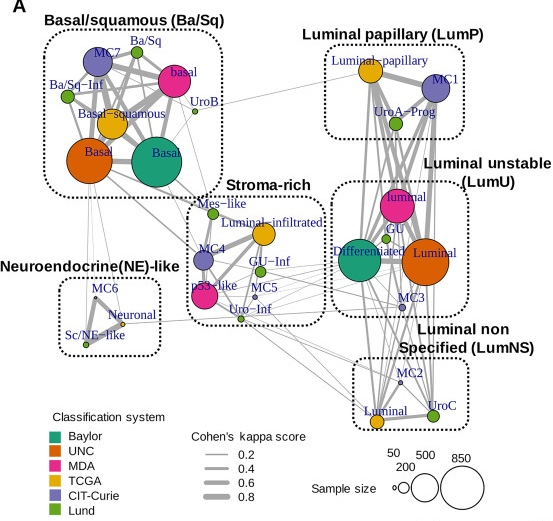
\includegraphics[width=0.6\textwidth,height=0.6\textheight,keepaspectratio]{Sections/Lit_review/Resources/consensus_network_classifier.jpg}
    \caption[Network of the datasets involved in the MIBC consensus]{Grouping the different MIBC classifier using the network approach described in \cite{Guinney2015-fy}. There are six main groups, characterised in \cref{fig:lit:2020_consens}. \acrfull{ba/sq} is the largest group which is also the second most aggressive subtype. Another major subtype is represented by the Luminal: papillary, unstable and non-specified, Stroma-rich contains most previous subgroups that contained infiltration. The smallest group is \gls{NE} and it encompass the most aggressive MIBC tumours. Image adapted from the consensus work \citet{Kamoun2020-tj}.}
    \label{fig:lit:consensus_network}
\end{figure}




% Other omics in bladder cancer
\subsection{The multi-facets of bladder cancer} \label{s:lit:bladder_other}

% Some properties of the bladder cancer
% - highly mutated, a lot of epginetic changes
Mutational signature are patterns of change in the DNA which are caused by different factors such as ageing, smoking and environmental hazards (arsenic contamination). The mutation signatures across human tumour types were collected and presented in the work of \citeauthor{Alexandrov2013-gi}, covering approximately 7000 cancer samples from which 20 distinct mutational signatures were extracted. \Cref{fig:lit:cancer_mut_sig} illustrates the mutation burden across tumour types, with skin cancer being the most mutated. Bladder cancer has the fourth highest mutation burden with Signatures 13, 2, and 5 from the COSMIC database \citep{Tate2019-yj}, these are shown in \cref{fig:lit:bladder_mut_sig}. Signatures 2 and 13 are related to APOBEC family activity, which is triggered by genomic instability \citep{Baker2022-xw}. Signature 5 is denotes mutation accumulated through ageing but the cause of it has not been proven. As MIBC classifiers primarily use gene expression for subtyping, the high mutation burden of MIBC highlights the lost potential in improving disease subgroups by using multiple data types.

\begin{figure}[!t]    
    \centering
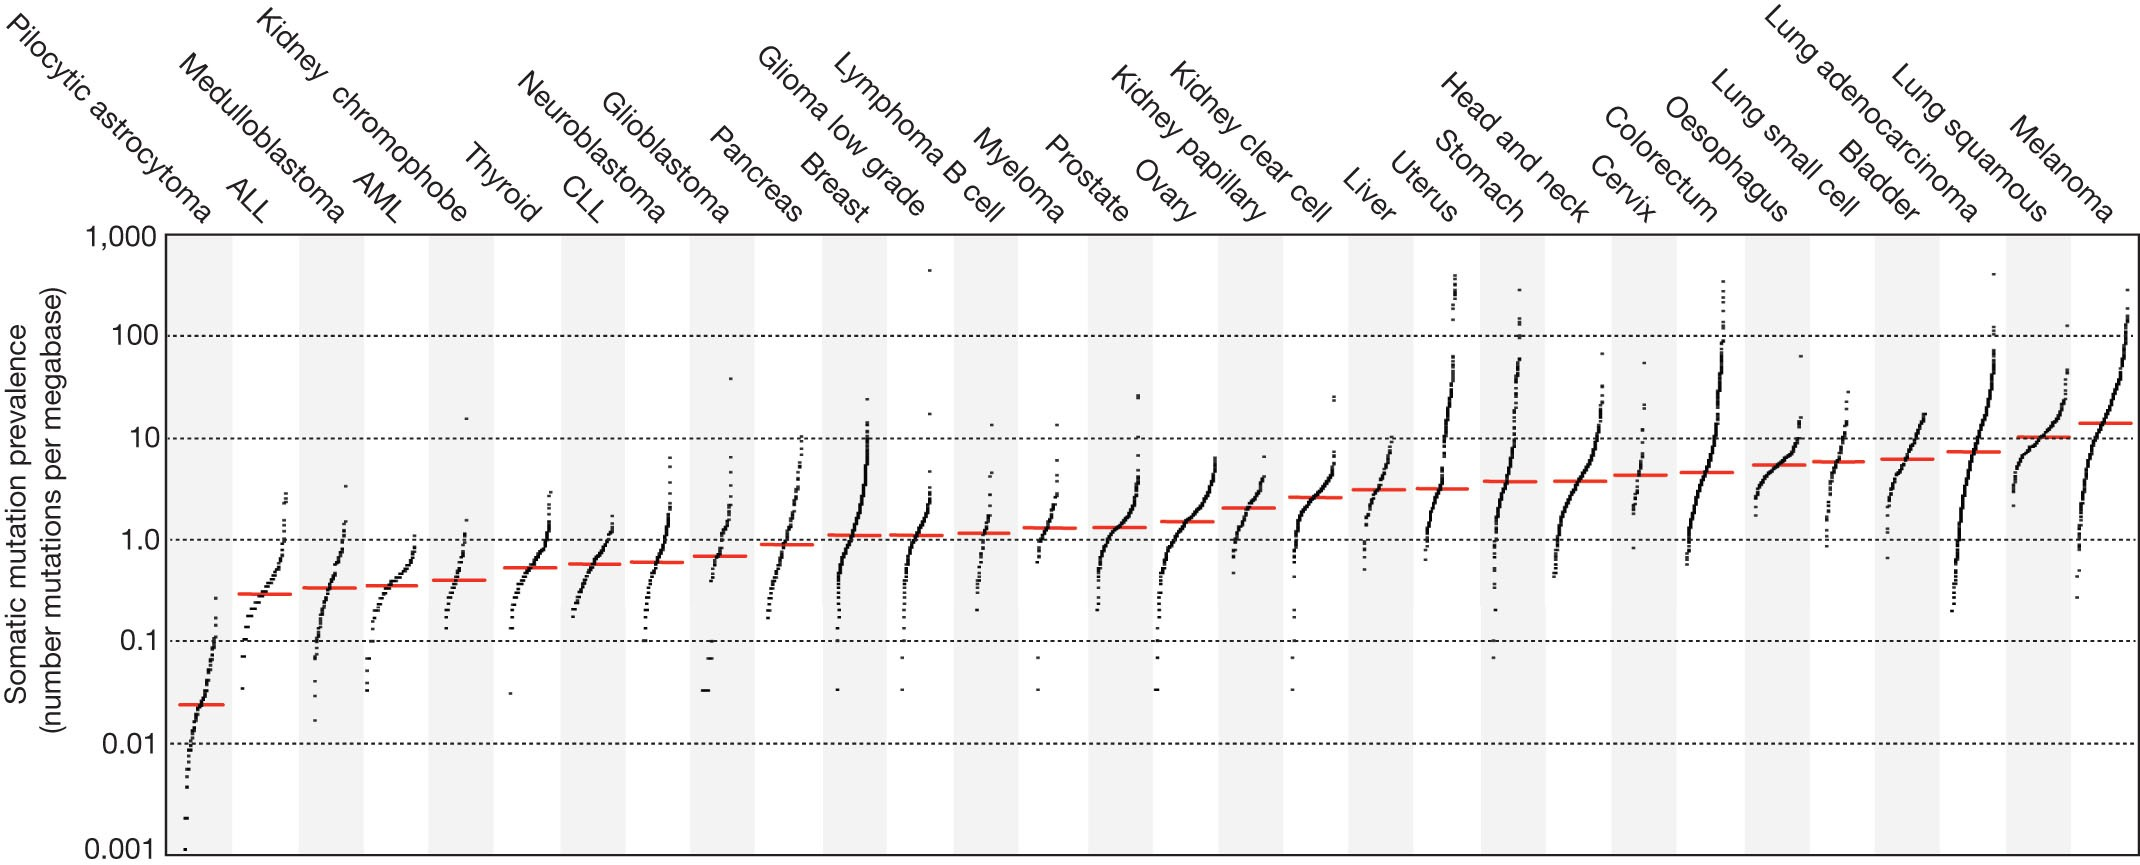
\includegraphics[width=0.9\textwidth,height=0.9\textheight,keepaspectratio]{Sections/Lit_review/Resources/mut_sig_cancers.jpg}
    \caption[Somatic mutations across human cancers]{Image from \cite{Alexandrov2013-gi} showing somatic mutations across different human cancers. Each sample is represented by a dot, and the red line indicates the median number of mutations in that tumour type. The y-axis shows the number of mutations per megabase, with cancer types ordered by the median mutation count, placing bladder cancer as the fourth highest mutated cancer. Image reproduced from \citep{Alexandrov2013-gi}, license: 5863680168690. }
    \label{fig:lit:cancer_mut_sig}
\end{figure}

% Epigenetic burden
The high somatic mutation burden is also emphasised in stratification studies \citep{Tcga2014-dr, Robertson2017-mg, Kamoun2020-tj}. A high mutation burden increases the disease's complexity, making it more difficult to understand because of higher heterogeneity and more gene mutation drivers. The two studies \citep{Tcga2014-dr, Robertson2017-mg} found that mutations also disrupt the epigenetic machinery. The disruption at different molecular levels makes the bladder complex, and it only reinforces the project's hypothesis to build an integrative method to inform MIBC stratification. Analysing the anomalies at the different molecular levels together can help the understanding of bladder tumours and develop new targeted treatments.


\begin{figure}[!htb]    
    \centering
    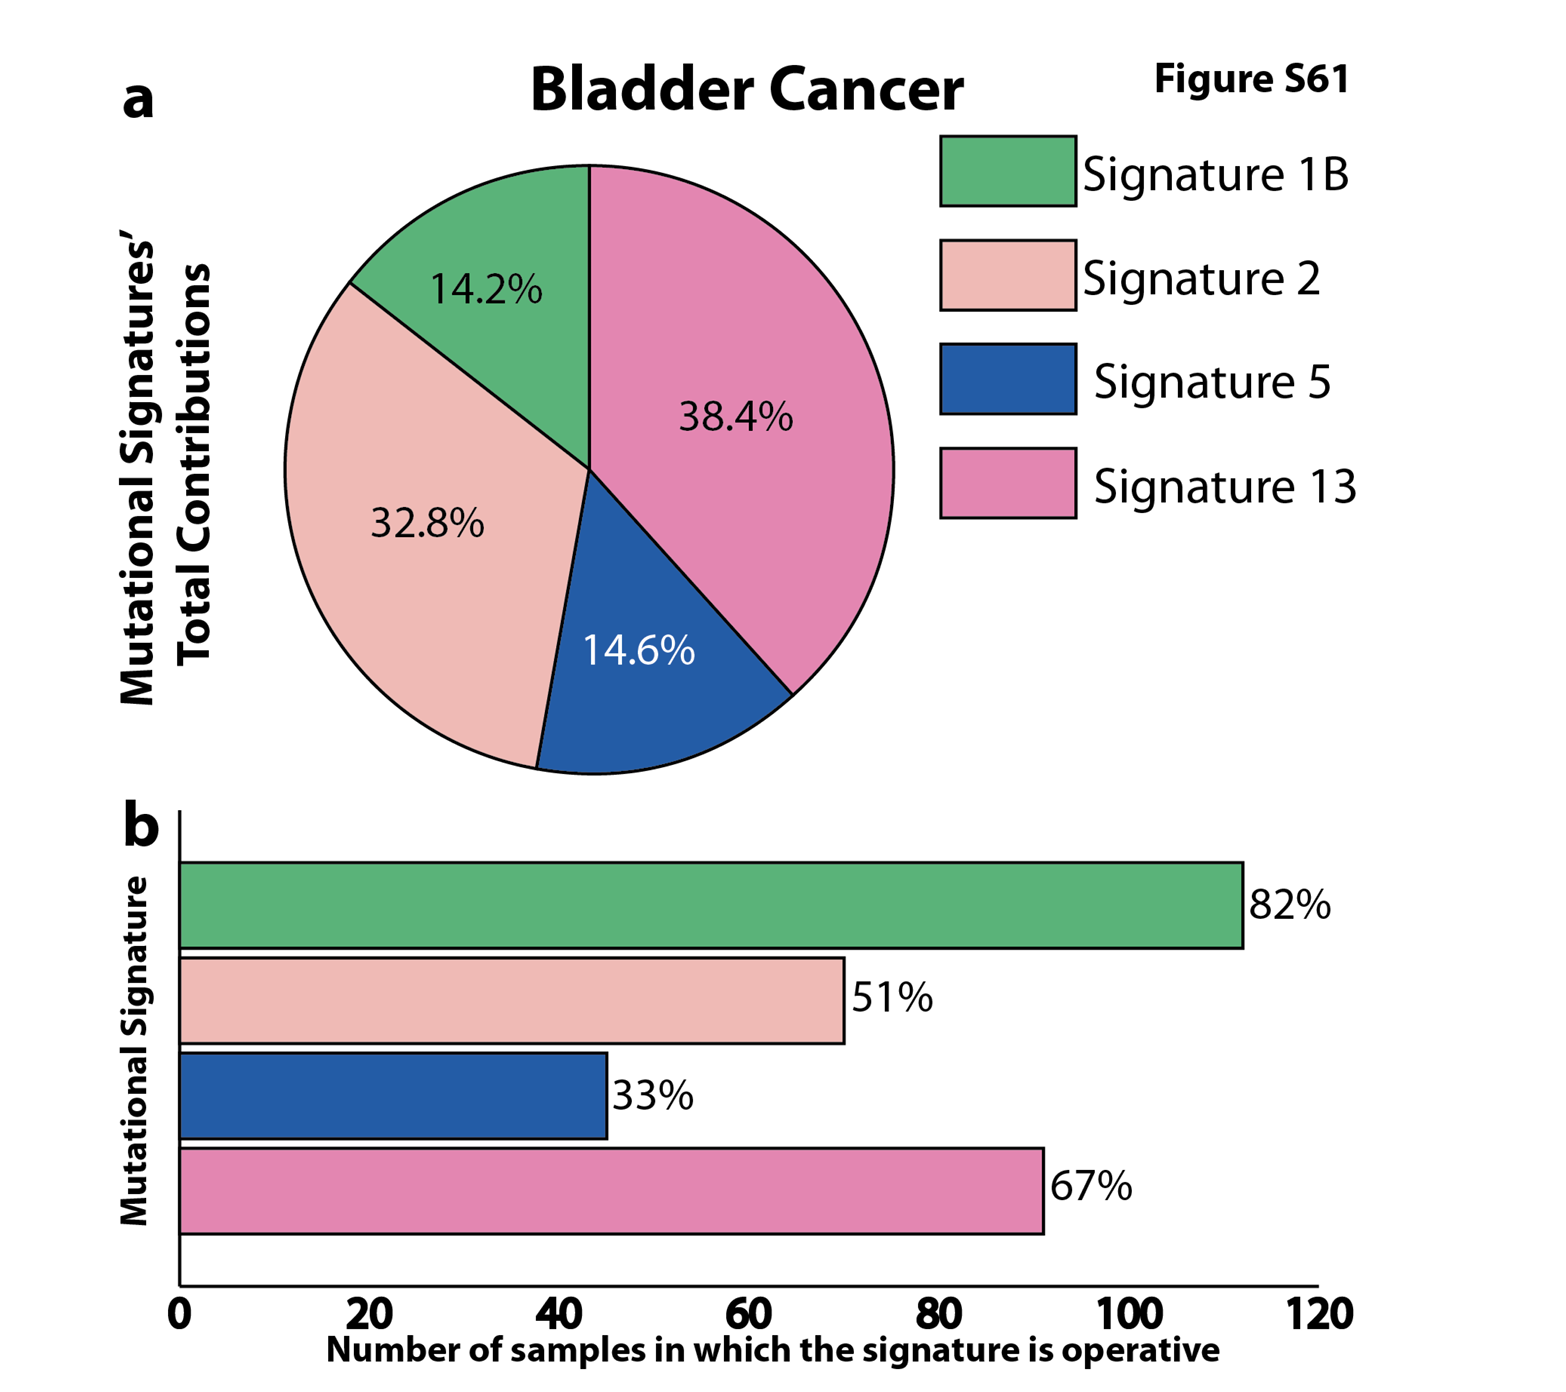
\includegraphics[width=0.6\textwidth,height=0.6\textheight,keepaspectratio]{Sections/Lit_review/Resources/bladder_mut_sig.png}
    \caption[Bladder mutational signature]{Image from the supplementary material from \citeauthor{Alexandrov2013-gi} showing the mutation signatures for bladder cancer. Panel (a) displays the contribution of each signature while panel (b) shows the number of samples where it was found. The image shows the high Tumour mutation burden of the bladder cancer compared to the others. Image reproduced from \citep{Alexandrov2013-gi}, license: 5863680168690. }
    \label{fig:lit:bladder_mut_sig}
\end{figure}



\subsection{Clinical translation} \label{s:lit:clinical}


The MIBC heterogeneity and the challenging aspect of finding clinically relevant subgroups is also shown in the subsequent work from \citeauthor{Robertson2023-na}, the lead author in TCGA study. The more recent study concentrates on a smaller cohort of 82 patients who underwent pembrolizumab treatment\footnote{This is a type of immunotherapy offered to patients with advanced MIBC and metastatic,} with the purpose of understanding the molecular profiles of the aggressive tumours that do not respond to traditional treatments. The pre-treatment tumour samples were clustered in five different subtypes each with different recurrence rate (\cref{fig:lit:immune_rob}). S3, S2 and S5 exhibited the highest response (A) to the treatment which also had the best \textbf{no} recurrence rate (B). \Cref{fig:lit:immune_rob} (C) shows how the five groups in \cite{Robertson2023-na} are classified by the existing classifications: TCGA, Consensus, Lund and MD Aderson \citep{Robertson2017-mg,Kamoun2020-tj,Marzouka2018-ge,Dadhania2016-cb}. 

Despite the fact that \citeauthor{Robertson2023-na} found statistical significance similarities between the immune therapy response groups and the other classifications, the five subtypes exhibit new properties and were not clearly situated in the previous groups (\cref{fig:lit:immune_rob}) (C), particularly S3 or S4 subgroups which are not easily identifiable with one of the previous subtypes. This highlights the challenging aspect of the MIBC stratification.


\begin{figure}[!htb]    
    \centering
    \includegraphics[width=0.9\textwidth,height=0.9\textheight,keepaspectratio]{Sections/Lit_review/Resources/robetson_summary_immune.png}
    \caption[MIBC subtypes based on the response to immunotherapy]{Adapted version of Figure 1 from \cite{Robertson2023-na} showing the 82 pre-treatment samples clustered in the five discovered groups. A) Showing the response to the immune treatment split in three categories: complete response (CR), partial response (PR) and non-response (NR). S3 having the best response followed by S2 and S5. B) The recurrence rate of the MIBC in the five groups, S5, S2 and S3 showing the highest \textbf{no} recurrence rate C) How are the five groups classified by the other grouping conventions.}
    \label{fig:lit:immune_rob}
\end{figure}


There is currently an ongoing clinical trial, GUSTO (gene expression subtypes of \gls{UC}: Stratified Treatment and Oncological outcomes), which uses TCGA subtypes to determine the treatment for patients suffering of aggressive bladder cancer. The study is based in the UK, consists of 320 patients over 3 years, and uses a commercially available MIBC test called Decipher Bladder\footnote{See \url{https://www.veracyte.com/decipher-bladder/}} with TCGA subtypes \citep{Griffin2024-zr}. The patients are randomised, with some  due to receive the standard treatment while others the treatment specific to their disease subtype. There are three different plans for Basal \& Neuronal, Luminal infiltrated, and Luminal Papillary \& Luminal.

The above two translational clinical efforts highlight the weight of TCGA study from \citet{Robertson2017-mg} in bladder classification, especially given that the GUSTO trial has used TCGA classifier over the consensus and the Lund cohort, which had the IHC information. It also underlines the importance of a good classifier and of having well-defined clusters. For example, the LumInf subtype (by TCGA) has its own immunotherapy treatments in the GUSTO trial but there is a large variance between the consensus, TCGA and Lund classifiers (\cref{fig:lit:classifier_comp}). This is a strong motivator for the project and for combining multiple data types at the computational level.



% Aims & Objective
% \subsection{Aims \& Objectives} \label{s:lit:aims_objs}

\subsection{Summary}

Multiple studies have been presented throughout this section, all with the singular aim of stratifying muscle-invasive bladder cancer to identify clinically relevant subtypes. The large number of studies addressing the same issue foregrounds the importance of understanding and treating MIBC, highlighting the disease's complexity. Earlier works by the Lund group \citep{Sjodahl2017-xr,Marzouka2018-ge} and TCGA \citep{Tcga2014-dr,Robertson2017-mg} presented subtypes with clear markers. However, in the later MIBC consensus work \citep{Kamoun2020-tj} which includes the aforementioned studies—there is a less clear description of MIBC subtypes. The ambiguity reinforces the heterogeneity and challenges of studying MIBC.

The studies considered in the MIBC consensus employ a similar cluster analysis process: data preprocessing, dimension reduction, and then hierarchical clustering. This analysis is applied solely to gene expression data. Consequently, the MIBC subtypes are based on a single type of data and derived from similar computational methods.

The following sections introduce the methods \& datasets used throughout the project (in \cref{s:lit:computational}), a literature review of the research efforts to stratify the \acrshort{mibc} and other diseases, either on single-omics or using integrative methods (in \cref{s:lit:multi-omics}). Lastly, the chosen computational methods, networks (\cref{s:lit:nets_bio}), and community detection (\cref{s:lit:comm_detect}), are explained in the last two parts of the chapter. The network and community detection sections provide important background for the experiments performed in \cref{s:N_I} and \cref{s:N_II}. The cluster analysis section is central to \cref{s:clustering_analysis}, which demonstrates that by applying simple algorithms to TCGA cohort, new biologically relevant subtypes are identified.



% This project addresses the limitations of the previous studies by introducing an integrative network approach, iNet, with the following aims: 1) create a method that allows the integration of multiple data types, 2) enable researchers to trace the biology behind each subtype, and 3) use non-cancerous gene expression to inform the tumour classifications. The underlying hypothesis is that integrating multiple data types, such as somatic mutations or prioritising Transcription Factors (TF), will yield clearer subtypes. Additionally, it is hypothesised that focusing on data from truly normal non-cancerous dataset can reveal new biology on the tumour subtyping.

% The objectives, or requirements, of the iNet approach are: 1) to be computationally simple, the complexity should arise from the biology, 2) to help trace genes contributing to different subtypes, 3) to create a platform that will enable the integration of more data types than those considered in this PhD project, and 4) to ensure the method is modular and data-agnostic, allowing its application to cancers from other tissues
